\section{Misura della lunghezza d'onda di un laser verde}
Dopo aver effettuato la calibrazione dell'apparato, ci è stato permesso testare lo strumento per la misurazione della lunghezza d'onda ignota di un secondo laser di colore verde.

Abbiamo nuovamente contato il numero di frange passanti per un riferimento scelto. Successivamente abbiamo ricavato il valore di lambda attraverso la relazione
\begin{equation}
    \lambda=\dfrac{2\cdot d\cdot \cos\theta}{N}
\end{equation}
\noindent
Le tabelle che seguono riportando i conteggi del numero di frange $\Delta N$ e il corrispondente valore $\lambda$

\begin{table}[h!]
    \centering
    \begin{tabular}{ccc}
    & Numero di frange\\
    \hline
         & 71 & 73\\
         &76 &75\\
         &71 &78\\
         &81 &73\\
         &77 &74 \\
    \hline\hline
    \end{tabular}
    \qquad\qquad
    \begin{tabular}{ccc}
    &\lambda\,nm\\
    \hline
         & 563,37 & 547,94 \\
         & 526,31 & 533,33 \\
         & 563,37 & 512,81 \\ 
         & 493,82 & 547,94 \\
         & 519,47 & 540,53 \\
    \hline\hline
    \end{tabular}
    \caption{}
\end{table}
\FloatBarrier
\noindent
\begin{figure}[h!]
    \centering
    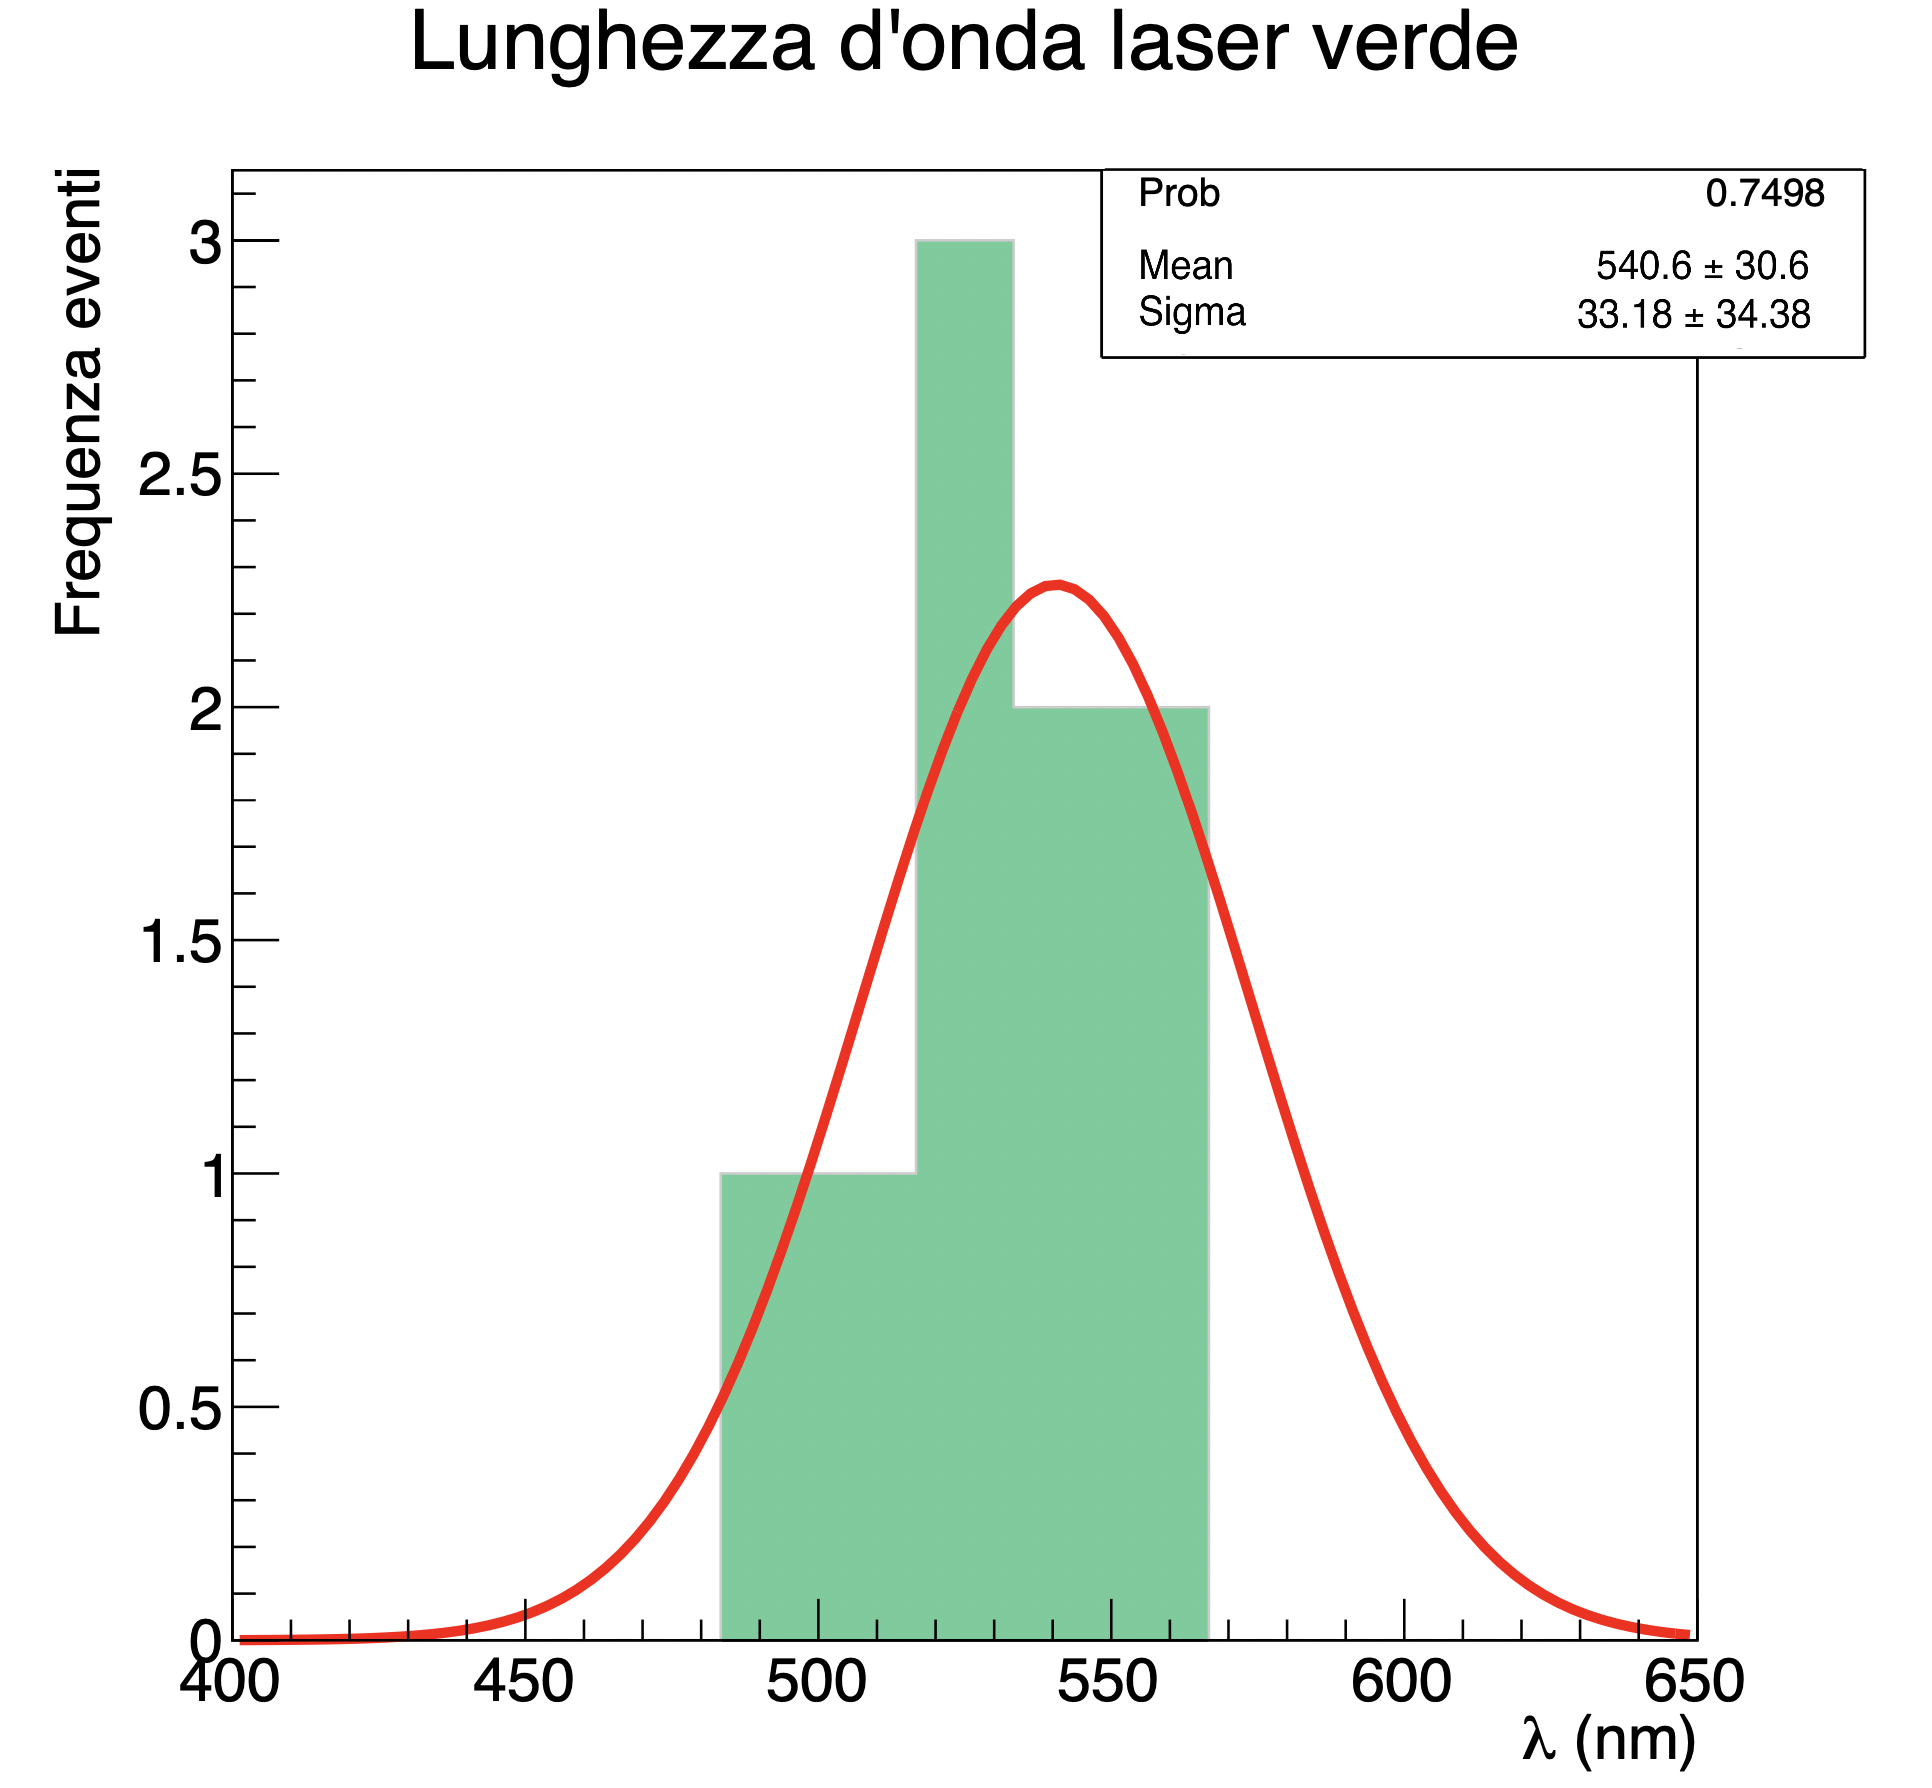
\includegraphics[scale=.33]{immagini/verde.png}
    \caption{}
    \label{fig:my_label}
\end{figure}
Il valore trovato è $\lambda = 534,89\, \pm 23,18\, nm$.











